% Figura 5 do Cap. I: etapas de aplicação do ARIMA. Substitui o PNG antigo em
% 27/10/2026, a pedido do autor (alternativa A1 de
% notas/rascunhos/diagramas_2026-10-27/alternativas_v1.pdf, com "real menos
% previsto" no lugar de "entrada do GARCH"). Compilada pelo Makefile do tg/.
\documentclass[11pt,border=2pt]{standalone}
\usepackage[T1]{fontenc}
\usepackage[utf8]{inputenc}
\usepackage{mathptmx}
\usepackage{tikz}
\usetikzlibrary{arrows.meta,positioning,calc,shapes.geometric,decorations.pathreplacing}
\tikzset{
  seta/.style={-{Stealth[length=2.2mm]}, semithick},
  caixa/.style={rectangle, draw, semithick, fill=gray!10, rounded corners=2pt,
                align=center, minimum width=54mm, minimum height=9mm, font=\small},
  caixap/.style={caixa, minimum width=32mm},
  decisao/.style={diamond, draw, semithick, fill=white, aspect=2.6, align=center,
                  inner sep=1pt, font=\small},
  dado/.style={trapezium, trapezium left angle=75, trapezium right angle=105, draw,
               semithick, fill=white, align=center, minimum height=9mm, font=\small,
               trapezium stretches body},
  rotulo/.style={font=\footnotesize\itshape, align=center},
}
\begin{document}
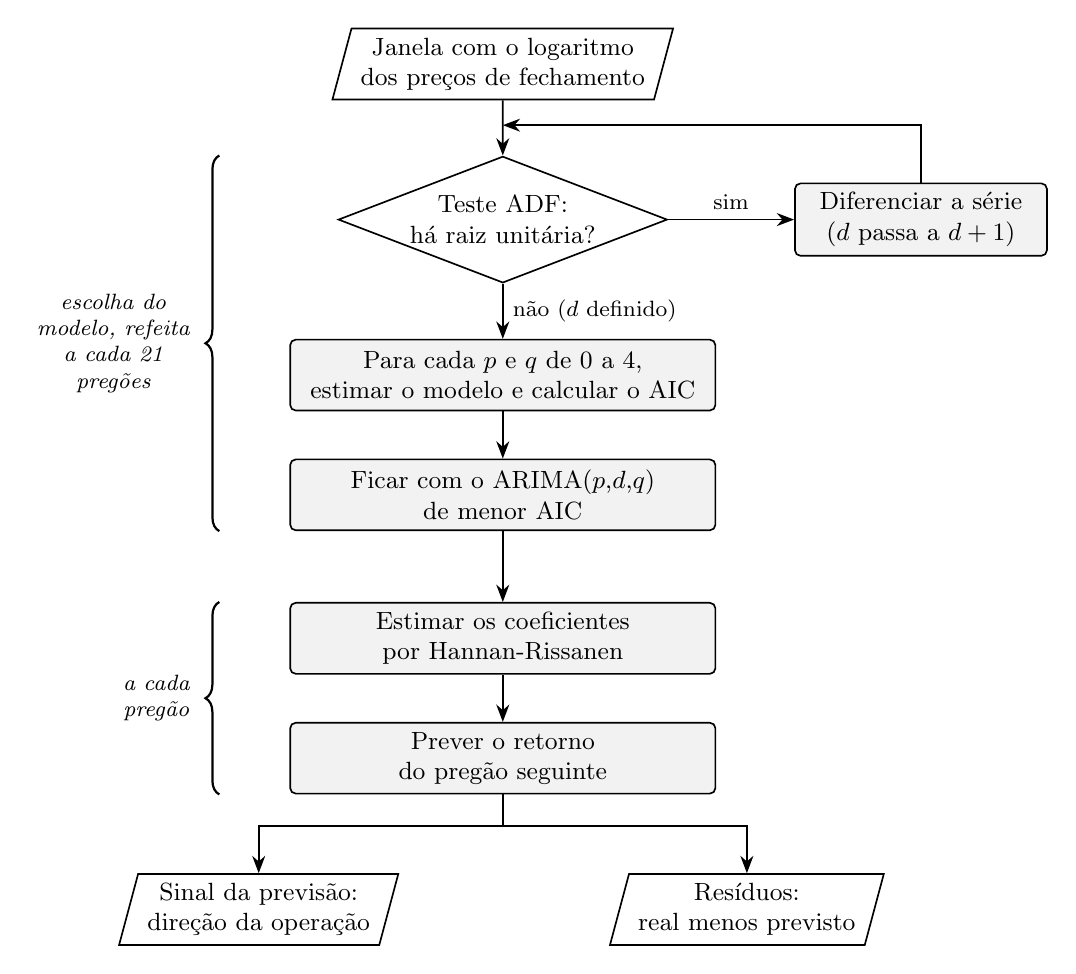
\begin{tikzpicture}[node distance=6mm]
  \node[dado] (ent) {Janela com o logaritmo\\dos preços de fechamento};
  \node[decisao, below=7mm of ent] (adf) {Teste ADF:\\há raiz unitária?};
  \node[caixap, right=16mm of adf] (dif) {Diferenciar a série\\($d$ passa a $d+1$)};
  \node[caixa, below=7mm of adf] (grade) {Para cada $p$ e $q$ de 0 a 4,\\estimar o modelo e calcular o AIC};
  \node[caixa, below=of grade] (esc) {Ficar com o ARIMA($p$,$d$,$q$)\\de menor AIC};
  \node[caixa, below=9mm of esc] (est) {Estimar os coeficientes\\por Hannan-Rissanen};
  \node[caixa, below=of est] (prev) {Prever o retorno\\do pregão seguinte};
  \node[dado, below=10mm of prev, xshift=-31mm] (dir) {Sinal da previsão:\\direção da operação};
  \node[dado, below=10mm of prev, xshift=31mm] (res) {Resíduos:\\real menos previsto};

  \coordinate (volta) at ($(ent.south)!0.45!(adf.north)$);
  \draw[seta] (ent) -- (adf);
  \draw[seta] (adf) -- node[above, font=\footnotesize]{sim} (dif);
  \draw[seta] (dif.north) |- (volta);
  \draw[seta] (adf) -- node[right, font=\footnotesize]{não ($d$ definido)} (grade);
  \draw[seta] (grade) -- (esc);
  \draw[seta] (esc) -- (est);
  \draw[seta] (est) -- (prev);
  \draw[seta] (prev.south) -- ++(0,-4mm) -| (dir.north);
  \draw[seta] (prev.south) -- ++(0,-4mm) -| (res.north);

  \draw[decorate, decoration={brace, amplitude=5pt, mirror}, thick]
    ([xshift=-36mm]adf.north) -- ([xshift=-36mm]esc.south)
    node[midway, left=7pt, rotulo]{escolha do\\modelo, refeita\\a cada 21\\pregões};
  \draw[decorate, decoration={brace, amplitude=5pt, mirror}, thick]
    ([xshift=-36mm]est.north) -- ([xshift=-36mm]prev.south)
    node[midway, left=7pt, rotulo]{a cada\\pregão};
\end{tikzpicture}
\end{document}
